\input{../../input/main}

\usetikzlibrary{hobby}

\begin{document}

\begin{center}
  \Large{\textbf{Городской центр физического образования, 10 класс.}\\
  \textit{Серия 8, 13 ноября 2014.}}
\end{center}

\begin{center}
  \Large \textbf{ Псевдоолимпиада. }
\end{center}

\large

\task{ Частица движется вдоль прямой. На ее пути на равных расстояниях
  $L$ друг от друга располагаются ловушки. Между ловушками частица
  разгоняется с постоянным ускорением $a$. Попадая в ловушку, частица
  мгновенно останавливается, после чего сразу же начинает новый
  разгон. Определите среднюю скорость частицы за время много большее
  времени движения между ловушками. Постройте график зависимости
  средней скорости от величины ускорения $a$.  }
% СПб, район-10, 2013

\taskpic{ На шероховатом полу около вертикальной гладкой стены стоит
  ящик массой $M$. Однородный массивный стержень \textbf{OA} шарнирно
  прикреплен к ящику в точке \textbf{O}. Определите при каких
  значениях коэффициента трения ящика о пол $\mu$, система будет
  оставаться неподвижной. Масса стержня $m$, расстояние от шарнира до
  стены равно $a$, расстояние от точки \textbf{A} до ящика равно
  $b$. Трением в шарнире пренебречь. }
{
  \begin{tikzpicture}
    \draw[fill=gray!40] (0,0) rectangle (2,1); 
    \draw[very thick,interface] (2.5,0) -- (0,0);
    \draw[very thick] (0,0) -- (0,2);
    \draw[very thick] (1,1) node[above] {\textbf{O}} -- (0,1.5) node[above
    right] {\textbf{A}}; 
    \draw[fill=black] (1,1) circle (0.05cm);
    \draw[thick,blue,<->] (1,0.6) -- (0,0.6) node[midway,blue,below]
    {$a$};
    \draw[blue,thick,<->] (-0.2,1.5) -- (-0.2,1) node[midway,left] {$b$}; 
  \end{tikzpicture}
}
% СПб, район-10, 2013

\taskpic{ Электрический нагреватель состоит из двух параллельных
  стержней длиной $2L$, расположенных на расстоянии $2a$, и регулятора
  \textbf{AB}, способного вращаться вокруг точки
  \textbf{O}. Сопротивление каждого стержня $R=100$ Ом, регулятор
  имеет нулевое сопротивление. Стержни подключены к источнику
  постоянного тока с напряжением $U=210$ В, как показано на
  рисунке. При помощи этого нагревателя воду массой $M=2$ кг доводят
  от температуры $T_0=16^{\circ}\,\mathrm{C}$ до кипения. Найдите зависимость
  времени кипячения воды $t$ от угла $\phi$, который регулятор
  образует с горизонталью, и постройте график зависимости $t$ от
  величины $\mathrm{tg}\, \phi$. Удельная теплоемкость воды
  $c=4200\mbox{ Дж}/\mbox{кг} \cdot {}^{\circ} \mathrm{C}$.  Теплопотерями и
  сопротивлением проводов пренебречь, $L=20$ см, $a=10$ см. }
{
  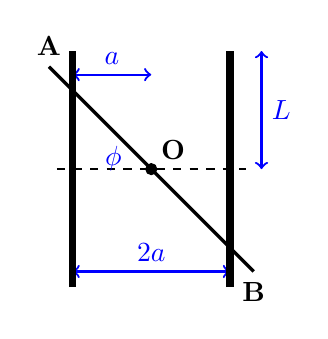
\begin{tikzpicture}
    \draw[blue,thick,<->] (0,0.2) -- ++(2,0) node[midway,above]
    {$2a$}; 
    \draw[blue,thick,<->] (2.4,3) -- (2.4,1.5) node[midway,right]
    {$L$};
    \draw[blue,thick,<->] (0,2.7) -- (1,2.7) node[midway,above] {$a$};
    \draw[dashed,thick] (-0.2,1.5) -- (2.2,1.5);
    \draw[line width=0.1cm] (0,0) -- (0,3) (2,0) -- (2,3);
    \draw[fill=black] (1,1.5) circle (0.07cm) node[above right]
    {\textbf{O}}; 
    \draw[very thick] (-0.3,2.8) node[above] {\textbf{A}} -- (2.3,0.2)
    node[below] {\textbf{B}};
    \draw (1,1.5) ++(165:0.5cm) node[blue] {$\phi$}; 
  \end{tikzpicture}
}
% СПб, район-10, 2010

% \taskpic{ В стакане с вертикальными стенками находятся вода и
%   примерзший ко дну лед. На поверхности воды строго горизонтально
%   плавает зеркало, на которое светят лазерной указкой под углом
%   $\alpha$. В стакан начинают наливать воду при температуре
%   $T$. Найдите скорость зайчика на потолке $v$, если в единицу времени
%   в стакан поступает объем воды $\mu$. Положение и ориентация указки
%   не изменяются. Считайте, что система в любой момент времени
%   находится в состоянии теплового равновесия, теплопотерями
%   пренебречь. Площадь дна стакана $S$, удельная теплота плавления льда
%   $\lambda$, удельная теплоёмкость воды $c$, плотность воды
%   $\rho_{\mbox{в}}$, плотность льда $\rho_{\mbox{л}}$.  }
% {
%   \begin{tikzpicture}
%     \draw[interface,thick] (3.6,0) -- (0,0);
%     \draw[fill=gray!80] (0.5,0) rectangle (3,0.7) node[midway] {лёд};
%     \draw[fill=gray!20] (0.5,0.7) rectangle (3,1.4) node[midway] {вода}; 
%     \draw[thick] (0.5,2) -- (0.5,0) -- (3,0) -- (3,2);
%     \draw[line width=0.07cm] (1,1.435) -- ++(1,0);
%     \begin{scope}[rotate around={45:(1.5,1.435)}]
%       \draw[thick] (2.3,1.435) rectangle ++(0.7,0.3);
%     \end{scope}
%     \draw[thick] (1.35,1.435) -- ++(45:0.9cm);
%     \draw[thick] (1.35,1.435) -- ++ (135:1.5cm);
%     \draw[thick,interface] (0,2.5) -- ++ (1,0);
%     \draw[very thick,->] (3.2,2.5) node[above,blue] {$\mu$}
%     to[out=200,in=80] (2.7,1.5);
%     \draw (1.5,1.435) ++ (35:0.3cm) node[blue] {$\alpha$}; 
%   \end{tikzpicture}
% }



\end{document}


%%% Local Variables: 
%%% mode: latex
%%% TeX-engine:xetex
%%% TeX-PDF-mode: t
%%% End:
